\chapter{Mathematical Formulation}
\label{mathchapter}

The objective of this fake thesis document is to demonstrate
a multitude of \LaTeX{} features as well as features specific
to the thesis class.
We start by giving one short formula,
and one big hairy multi-line formula
(one of the non-dimensional Navier-Stokes equations):


\begin{equation}
	A = \pi r^2
\end{equation}


\begin{eqnarray}
  \rho \left[ \frac{DV_r}{Dt} - M \epsilon^2
    \frac{\vth^2}{r} \right]
  & = & -\frac{\delta^2}{\gamma~ M} \diffr{P}
	+ \frac{M ~\delta^2}{Re} \left\{ 2 \diffr{}
	\left[ \mu \left( \diffr{V_r}
        - \frac{1}{3} {\bf \nabla \cdot \overline{V}}
      \right) \right] \right. \nonumber \\
  & & + \frac{1}{r} \diffth{} \left[ \mu \left(
      \frac{1}{r} \diffth{V_r} + \epsilon \diffr{\vth}
      - \epsilon \frac{\vth}{r} \right) \right] \nonumber \\
  & & + \diffz{} \left[ \mu \left( \frac{1}{\delta^2}
        \diffz{V_r} + \diffr{V_z} \right) \right] \nonumber \\
  & & + 2 \left. \frac{\mu}{r}\left[ \diffr{V_r} -\frac{\epsilon}{r}
      \diffth{\vth} - \frac{V_r}r\right] \right\}, \label{eq:rmom}
\end{eqnarray}


The latter equation is non-dimensionalized using the following definitions:

\[
	r = \frac{r'}{R'}, ~~~
	z = \frac{z'}{L'},~~~
	t = \frac{t'}{t_a'}, ~~~
	\kappa = \frac{\kappa'}{\kappa_0'}, ~~~
	\mu = \frac{\mu'}{\mu_0'} , ~~~
	C_V = \frac{C_V'}{C_{V0}'},
\]
where $P_0'$ is the initial static pressure in the cylinder,
and $\rho_0'$ and $T_0'$ are the density and temperature
of the fluid being injected from the sidewall.
The aspect ratio is given by $\delta = \frac{L'}{R'}$,
where $\delta \gg 1$.
The induced characteristic axial velocity and the characteristic
endwall velocity disturbance $V_{z0}'$ is defined with respect
to the injection reference sidewall velocity,
$V_{r0}'$ by overall mass conservation,
$\frac{V_{z0}'}{V_{r0}'} = \delta$.
The size of the initially unknown reference
azimuthal velocity $V_{\theta 0}'$ is related to
$V_{r0}'$ by $\frac{V_{\theta 0}'}{V_{r0}'}=\epsilon$.
Later, it is shown that $\epsilon=1$.

\begin{figure}
%\centerline{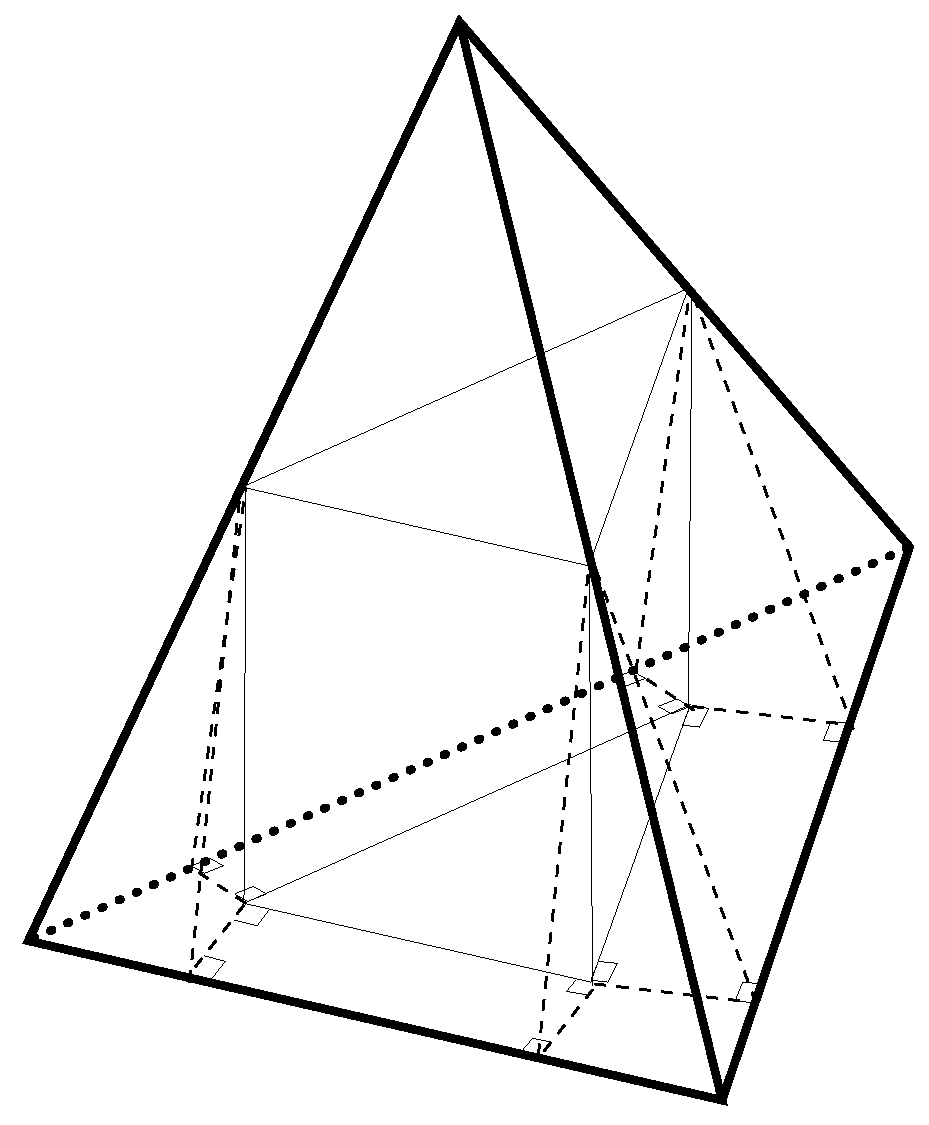
\includegraphics[height=95mm]{figures/pyr.ps}}
\caption[Cutting up a triangular pyramid]{
	A triangular pyramid may be cut up as shown, to
	yield one top pyramid (with one-eighth the volume
	of the full pyramid), three bottom corner pyramids
	(which, when joined, are congruent to the top pyramid),
	three prisms along the bottom edges (the area of whose
	bottom faces total $B/2$) and the large central prism
	(volume = $(B/4)(h/2) = Bh/8$).
	The image, from PostScript file ``pyr.ps'',
	was read in using the {\tt $\backslash$includegraphics}
	command, from the {\tt graphicx} package.
	}
\label{fig:pyramid}
\end{figure}


The time is non-dimensionalized using the
axial acoustic time scale,
$t_a'=\frac{L'}{C_0'}$, where
$C_0'=(\gamma {\cal R} ' T_0')^{\frac12}$
is the speed of
sound\footnote{In air at 1 atm., $\frac{1 mi.}{5 s}$.},
$\cal{R}'$ is the gas constant,
and $\gamma$ is the ratio of specific heats.
Also the Reynolds number, Wrenchl number,
and Mock number are defined as

\[
	Re = \frac{\rho' V_{z_0}' L'}{ \mu_0'}, ~~~
	Wr = \frac{\mu_0' C_{p_0}'}{\kappa_0'}, ~~~
	M = \twovec{V_{z_0}'}{C_0'} \cdot
		\twomatrix{8a}{z_0-\rho}2{z_0-\mu} \twovec{Wr}{p-7}
\]
where $Re\ll1$, $M\gg1$, and $Wr=O(1)$.

Here is an example of using the macros
\verb2\singlespacing2 and \verb2\doublespacing2:

\singlespacing	% <------------------------------

This paragraph was preceded by the
command \verb2\singlespacing2.
The Mock number is chosen as a small parameter to model the
small magnitude found in a typical rocket motor chamber,
as opposed to the rocket nozzle where larger values are
possible\footnote{Not just possible, desirable!}.
The aspect ratio, $\delta$, is taken to be
a large parameter, because many chambers
have aspect ratios between 15 and 50.
Now the command ``\verb2\doublespacing2'':

\doublespacing	% <------------------------------


The Grad School specifications allow for single spacing
everywhere in the body of the thesis, except in
quotations of four or more lines
(Dole and Abramson\cite{dole}),
table/figure captions, chapter headings, footnotes and
entries in the Contents and Bibliography
(with double spaces between entries).

And now, here is an example of using the macros
\verb2\begin{singlespace}2 and \verb2\end{singlespace}2;
another way to get single-spacing.

\begin{singlespace}	% <-----------------------------
Two cases are studied in the present work which differ only in the
boundary conditions.  Each different boundary condition model a
different source of instability.  The boundary of the first case
consists of a steady, axisymmetric sidewall radial velocity boundary
and a time-dependent, non-axisymmetric endwall axial velocity
boundary.  The second case is studied with a fixed impermeable axial
velocity along the endwall and a combination axisymmetric steady and
non-axisymmetric unsteady radial velocity along the sidewall.
\end{singlespace}	% <-----------------------------


Now on to other items.
The following table is created using \LaTeX{} macros,
i.e., \verb2\begin{tabular}2 \ldots \verb2\end{tabular}2.

\begin{table}
\begin{center}
\label{tbl:sample2}
\caption[Yet another {\tt tabular} table]{
	This is a table constructed with \LaTeX{}
	commands in the {\tt tabular} environment.
	}
   \begin{tabular}{|c||c|c|c|c||c|} \hline
   n & $n^2$ & $n^3$ & $n^4$  & $n^7$ & $n^{13}$ \cr \hline \hline
   2 &  4  &  8  &   16    &    128  & 8192 \cr
   3 &  9  &  27  &   81    &   2187  & 1594323 \cr \hline
   4 &  16  &  64  &   256   &  16384  & 67108864 \cr
   5 &  25  &  125  &   625  &  78125  & 1220703125 \cr \hline
   6 &  36  &  216  &   1296 &  279936  & 13060694016 \cr
   7 &  49  &  343  &   2401 &  823543  & 96889010407 \cr \hline
   \end{tabular}
\end{center}
\end{table}


However, sometimes you want to use a table produced by some other
software, such as Excel.  If the table is saved to a PostScript file,
then it can be displayed using the $\backslash${\tt includegraphics}
macro inside a {\tt table} environment:


\begin{table}
\caption[Table from a PostScript file]{
	This table wasn't constructed with \LaTeX{}
	commands, but resides in a PostScript file
	({\tt tableD.ps})
	created by some other software.
	}
\label{tbl:sample3}
%\centerline{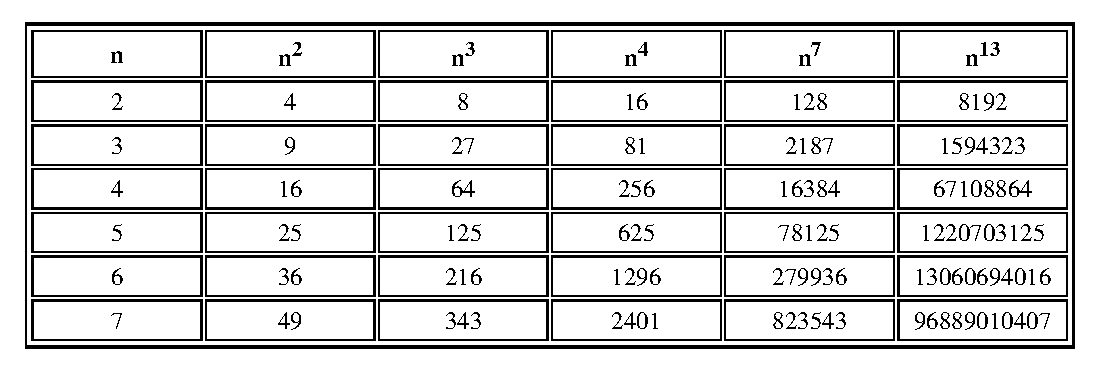
\includegraphics[width=4.45in]{figures/tableD.ps}}
\end{table}


\section{Conditions for Catastrophic Combustion}
\label{sec:cata}

Initially, a steady flow is generated by the sidewall
injection, $V_r = -V_{rws}(z)$.
The subscript $srw$ is used to mean that there is a
{\bf s}teady {\bf r}adial {\bf w}all velocity.
The sign is negative due to the injection toward centerline.
At $t=0^+$, the endwall begins oscillating with the
non-dimensionalized sinusoidal axial velocity,
$V_z=\widetilde{F}_{rw}(r,\theta,t)$,
for $\omega = O(1)$.
Figure \ref{fig:sidewaysF} conforms to these thesis specs:
``Figures are placed immediately after their first mentions \ldots
Figure captions appear below figures and are typed in the same
style and size as the text.  Captions should fit within the
standard margins and are not reduced if the figures are reduced
\ldots Figures may be printed broadside, with the top toward the
left margin; the caption then appears beneath the figure and is
typed from bottom to top of the page within the standard
margins\ldots''

\begin{sidewaysfigure}
\centerline{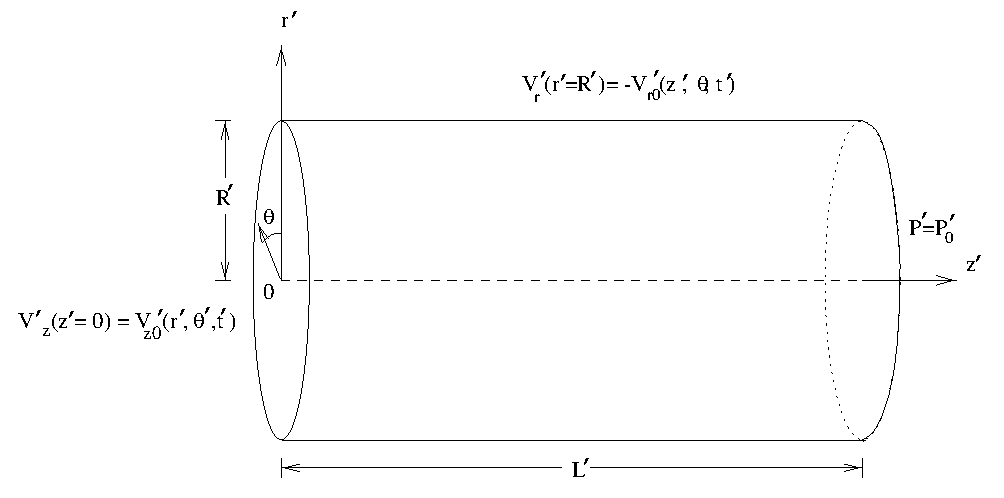
\includegraphics[width=7in]{figures/tube.eps}}
\caption[A Sideways Figure]{
	If a figure must appear sideways in a thesis
	(for greater detail) then the caption must still
	appear \emph{below} the figure --- i.e., along
	the right edge of the page.
	By including the \emph{rotating} package at the top of the
	\LaTeX{} file, you can get this rotated figure by using the
	{\tt $\backslash$begin$\{$sidewaysfigure$\}$} \ldots
	{\tt $\backslash$end$\{$sidewaysfigure$\}$} environment.
	}
\label{fig:sidewaysF}
\end{sidewaysfigure}



Some of the boundary conditions are:

\begin{eqnarray}
  z=0; && V_z = \twochoices
	{0, && t\leq0}
	{\widetilde{F}_{zw}(r,\theta,t), && t>0}
						\label{eq:endwall} \\
  z=0; && V_{\theta}=V_r=0			\label{eq:endnoslip} \\
  r=0; && P,\rho,T,V_r,\vth,V_z~\mbox{finite},	\label{eq:centerline} \\
  r=1; && V_r= F_{rws}(z),			\label{eq:injection} \\
  r=1; && V_z=\vth =0,				\label{eq:sidenoslip}
\end{eqnarray}
and solutions must be periodic in $\theta$.


\section{More Boundary Conditions}
\label{sec:bcs}

Initially, a steady flow is generated by the
sidewall injection, $V_r = -V_{rws}(z)$.
The sign is negative due to the injection toward
centerline\footnote{This convention was
suggested by Goddard and Smythe.}.
At $t=0^+$, the endwall begins oscillating with the
non-dimensionalized sinusoidal axial velocity,
$V_z =\widetilde{F}_{rw}(r,\theta,t)$,
for $\omega = O(1)$.
The frequency condition chosen represents the
first few axial acoustic modes observed in high
aspect ratio chambers\footnote{Toy rockets,
the kind you used to shoot off with your dad
in the park, typically have only two significant
modes.}.


The full boundary conditions include:

\begin{eqnarray}
  z=0; && V_{\theta}=V_r = 0            \label{eqB:endnoslip} \\
  r=1; && V_r= \left\{
    \begin{array}{ll}
      F_{rws}(z), & t<0, \\
      F_{rws}(z)+\widetilde{F}_{rw}(z,\theta,t) & t\geq 0
    \end{array}
  \right.                               \label{eqB:injection} \\
  r=1; && V_z=\vth =0,                  \label{eqB:sidenoslip}
\end{eqnarray}
and solutions must be periodic in $\theta$.


If you don't believe this stuff, check out
Mulick\cite{mulick} and Baylor\cite{baylor}.

The following two tables, and their respective captions,
are turned sideways.  They use the
\verb2sidewaystable2 environment defined in the
\verb2rotating2 package.  The first uses the \LaTeX{}
\verb2tabular2 environment, and would be used when the
normal \LaTeX{} table is a bit too wide to fit the
width of the page, but fits the page when rotated.
The second table is actually from a PostScript file,
perhaps produced by some other software.  It is read in
using the \verb2\includegraphics2 command, and is needed when the
table is very large and must be shrunk to fit the page.
Inside the \verb2\includegraphics2 command one can specify
{\tt width=8.75in}, which will scale the
(rotated) PostScript image to nearly fill the
maximum amount of vertical space on a thesis page.

\begin{quotation}
Tables are placed immediately after their first mention
in the text \dots Tables that will not fit within the
required margins may be typed in smaller type or may
be reduced; they also may be printed broadside with the
top toward the left margin \ldots Table titles are typed
above the tables in the same style and type size
as the text.  Table titles should fit within the
standard margins and are not reduced if the table
is reduced.  Table footnotes are typed immediately
beneath the table and have no relation to text footnotes.
\end{quotation}


\begin{sidewaystable}
\begin{center}
\caption[A sideways table with {\tt $\backslash$tabular}]{
	This sideways table is constructed using the
	{\tt $\backslash$tabular} environment.  This would
	only be necessary for tables so wide that they don't
	fit the normal width, but not so wide that they
	would also exceed 8.75", the usable height of a
	thesis page, using the usual \LaTeX{} font
	in the table.
	Notice that this table uses the same font
	style and size as in the body of the thesis.
	The caption appears \emph{above} the table
	(nearest the left edge of the page)
	as it should in a C.U.~thesis.
	}
   \begin{tabular}{|c||c|c|c|c||c|} \hline
   n & $n^2$ & $n^3$ & $n^4$  & $n^7$ & $n^{13}$ \cr \hline \hline
   2 &  4  &  8  &   16    &     128  & 8192 \cr
   3 &  9  &  27  &   81    &     2187  & 1594323 \cr \hline
   4 &  16  &  64  &   256    &     16384  & 67108864 \cr
   5 &  25  &  125  &   625    &     78125  & 1220703125 \cr \hline
   6 &  36  &  216  &   1296    &     279936  & 13060694016 \cr
   7 &  49  &  343  &   2401    &     823543  & 96889010407 \cr \hline
   100 & 10000 & 1000000 & 100000000 & 100000000000000 &
		100000000000000000000000000 \cr
   1000 & 1002001 & 1003003001 & 1004006004001 & 1007021035035021007001 &
		1013078286716288717717287715286078013001 \cr \hline
   \end{tabular}
\label{tbl:sidewaysL}
\end{center}
\end{sidewaystable}


\begin{sidewaystable}
\centering
\caption[A sideways table in a PostScript file]{
	This table is actually from a PostScript file.
	If it is just too tiny to read in the normal orientation,
	where the width is limited to 5.75",
	it can be displayed sideways at a width
	(vertical length) of up to 8.75".
	The contents of the table show that it has been
	reduced in size; however, the caption appears in
	the correct place above the table (left edge of page)
	in the same font style/size as in the body of the
	thesis.  The caption also appears in the list of
	tables at the front of the thesis.
	This construct uses the {\tt sidewaystable} environment
	and the {\tt $\backslash$includegraphics} command, which are
	defined in the \emph{rotating} and \emph{graphicx}
	packages, respectively.  These packages are read in
	(with {\tt $\backslash$usepackage})
	at the top of the \LaTeX{} file.
	}
\centerline{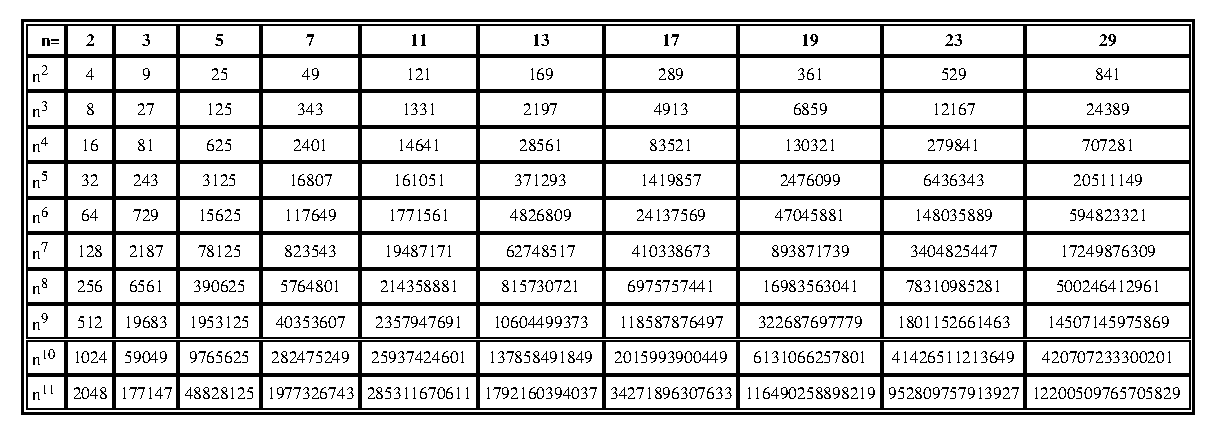
\includegraphics[width=8.75in]{figures/bigtable.eps}}
\label{tbl:sidewaysT}
\end{sidewaystable}



\subsection{
	Just meaningless text to test lines per page
	\label{ss}}

According to the Grad School specs.   there should be 24--27 lines
of print per page of a thesis.  This should be true whether the font
size is 10, 11, or 12.  Count them up; does this document conform?
According to the Grad School specs.   there should be 24--27 lines
of print per page of a thesis.  This should be true whether the font
size is 10, 11, or 12.  Count them up; does this document conform?
According to the Grad School specs.   there should be 24--27 lines
of print per page of a thesis.  This should be true whether the font
size is 10, 11, or 12.  Count them up; does this document conform?
According to the Grad School specs.   there should be 24--27 lines
of print per page of a thesis.  This should be true whether the font
size is 10, 11, or 12.  Count them up; does this document conform?
According to the Grad School specs.   there should be 24--27 lines
of print per page of a thesis.  This should be true whether the font
size is 10, 11, or 12.  Count them up; does this document conform?
According to the Grad School specs.   there should be 24--27 lines
of print per page of a thesis.  This should be true whether the font
size is 10, 11, or 12.  Count them up; does this document conform?
According to the Grad School specs.   there should be 24--27 lines
of print per page of a thesis.  This should be true whether the font
size is 10, 11, or 12.  Count them up; does this document conform?
According to the Grad School specs.   there should be 24--27 lines
of print per page of a thesis.  This should be true whether the font
size is 10, 11, or 12.  Count them up; does this document conform?
According to the Grad School specs.   there should be 24--27 lines
of print per page of a thesis.  This should be true whether the font
size is 10, 11, or 12.  Count them up; does this document conform?
According to the Grad School specs.   there should be 24--27 lines
of print per page of a thesis.  This should be true whether the font
size is 10, 11, or 12.  Count them up; does this document conform?
According to the Grad School specs.   there should be 24--27 lines
of print per page of a thesis.  This should be true whether the font
size is 10, 11, or 12.  Count them up; does this document conform?
According to the Grad School specs.   there should be 24--27 lines
of print per page of a thesis.  This should be true whether the font
size is 10, 11, or 12.  Count them up; does this document conform?
According to the Grad School specs.   there should be 24--27 lines
of print per page of a thesis.  This should be true whether the font
size is 10, 11, or 12.  Count them up; does this document conform?
According to the Grad School specs.   there should be 24--27 lines
of print per page of a thesis.  This should be true whether the font
size is 10, 11, or 12.  Count them up; does this document conform?
According to the Grad School specs.   there should be 24--27 lines
of print per page of a thesis.  This should be true whether the font
size is 10, 11, or 12.  Count them up; does this document conform?
According to the Grad School specs.   there should be 24--27 lines
of print per page of a thesis.  This should be true whether the font
size is 10, 11, or 12.  Count them up; does this document conform?
According to the Grad School specs.   there should be 24--27 lines
of print per page of a thesis.  This should be true whether the font
size is 10, 11, or 12.  Count them up; does this document conform?
According to the Grad School specs.   there should be 24--27 lines
of print per page of a thesis.  This should be true whether the font
size is 10, 11, or 12.  Count them up; does this document conform?
According to the Grad School specs.   there should be 24--27 lines
of print per page of a thesis.  This should be true whether the font
size is 10, 11, or 12.  Count them up; does this document conform?
According to the Grad School specs.   there should be 24--27 lines
of print per page of a thesis.  This should be true whether the font
size is 10, 11, or 12.  Count them up; does this document conform?


\paragraph{What is it?}
This is a labelled paragraph.
The heading of the paragraph is emphasized.
This is a labelled paragraph.
The heading of the paragraph is emphasized.

\subsection{This is a subsection}

This is a subsection.
Filler filler filler filler filler filler filler filler.
Filler filler filler filler filler filler filler filler.

\subsection{This is another subsection}

This is another subsection.
Filler filler filler filler filler filler filler filler.
Filler filler filler filler filler filler filler filler.

\paragraph{This is paragraph number 2.}
It used a \verb2\paragraph{}2 header, which
are always inlined (with extra space)
and  boldfaced.

This is the third paragraph of the subsection.
Filler filler filler filler filler filler filler filler.
Filler filler filler filler filler filler filler filler.


%%%%%%%%%%%%%%%%%%%%%%%%%%%%%%%%%%%%%%%%%%%%%%%%%%%%%%%%%%
%%%%%%%%%%%%%%%%%% SSSec 1 %%%%%%%%%%%%%%%%%%%%%%%%%%%%%%%
%%%%%%%%%%%%%%%%%%%%%%%%%%%%%%%%%%%%%%%%%%%%%%%%%%%%%%%%%%

\subsubsection{This is a subsubsection (1)}
This is the first paragraph of the subsubsection.
Whether it is numbered or inlined depends on the
option selected at the beginning of the
thesis.

By default, a \verb2\subsubsection2 heading is numbered
and set off on a separate line, left-justified.

\paragraph{However.}
Using the \verb2inlineh42 option, subsubsection headers
are inlined.
And using the \verb2nonumh42 option suppresses
numbering of the subsubsections.
Together they make subsubsection headings
just the same as paragraph headings.


%%%%%%%%%%%%%%%%%%%%%%%%%%%%%%%%%%%%%%%%%%%%%%%%%%%%%%%%%%
%%%%%%%%%%%%%%%%%% SSSec 2 %%%%%%%%%%%%%%%%%%%%%%%%%%%%%%%
%%%%%%%%%%%%%%%%%%%%%%%%%%%%%%%%%%%%%%%%%%%%%%%%%%%%%%%%%%

\subsubsection{
	This is another subsubsection (2)
	\label{sss}
	}

Once again, whether its heading is numbered
and/or inlined depends on the class options
chosen at the start.

There is no ``subsubsubsection'' entity,
and ``subparagraph'' gets no special treatment
in \emph{thesis} class.

\section{The End}
\label{sec:end}

Finally, this is the end.  The bibliography starts on
the next page.
